\ylDisplay{Peeglid} % Ülesande nimi
{Jaan Kalda} % Autor
{piirkonnavoor} % Voor
{2009} % Aasta
{G 8} % Ülesande nr.
{5} % Raskustase
{
% Teema: Geomeetriline-optika
\ifStatement
Kui paigutada kaks tasapeeglit nii, et nende tasapinnad moodustavad nurga $\alpha<180^\circ$ ning peegeldavad pinnad on vastamisi, siis peeglite vahele paigutatud asjadest võib tekkida mitu kujutist: lisaks peegeldustele veel peegelduse-peegeldused jne. Joonisel on kujutatud valgusallika $S$ kaks peegeldust ning üks peegelduse-peegeldus ülaltvaates (st peeglite tasapindade lõikejoone sihis). Leida konstruktsiooni abil peeglite ning valgusallika asukohad. Peeglitel on ainult üks peegeldav külg.\\

\begin{center}
	
\includegraphics[width=0.6\linewidth]{2009-v2g-08-yl}
\end{center}
\fi


\ifHint
Joonisel on kaks peegeldust ja üks peegelduse-peegeldus. Sellele vastab kolm võimalikku punktide konfiguratsiooni ning eeldatavasti on võimalik paari kavala argumendi põhjal osad konfiguratsioonid elimineerida (näiteks peab valgusallikas olema mõlema peegli vahel).
\fi


\ifSolution
%Ühe peegli (nimetagem seda \enquote{esimeseks} peegliks) tasandi saab leida peegelduse $S_1$ ning selle peegelduse peegelduse $S_1^\prime$ sümmeetriateljena.
%Seejuures $S_1$ on allika $S$ peegelduseks teises peeglis ning kolmas kujutis $S_2$ on seega allika peegeldus esimeses peeglis. Niisiis, olles leidnud esimese peegli, saame
%leida ka allika asukoha --- kujutise $S_2$ peegeldusena esimeses peeglis. Peale seda saab leida ka teise peegli --- $S$ ja $S_1$ sümmeetriateljena.
%Kujutiste paariks $S_1$ ja $S_1^\prime$ saab olla ainult kaks alumist punkti joonisel, sest vastasel korral jääks valgusallikas kõigi kujutiste suhtes teisele poole esimest peeglit;
%kuivõrd teine peegel jääb $S$ ja $S_1$ vahele, siis kehtib sama %ka teise peegli jaoks ja seega ei jääks $S$ peegite vahele. Niisiis, esimeseks peegliks on kahe alumise punkti sümmeetriatelg ning allikaks ülemise punkti peegeldus selles peeglis. Teine peegel peab olema allika ja parempoolse punkti sümmeetriatelg, sest kui see oleks allika ja vasakpoolse punkti sümmeetriatelg, siis jääks allikas jällegi peeglite vahelt välja
Kuna on teada, et üks antud punktidest on peegelduse peegeldus, siis peab üks tasapeeglitest kindlasti asuma peegelduse $S_1$ ning selle peegelduse peegelduse $S_1^\prime$ sümmetriateljel. Lisaks saab punkt $S_1$ tekkida ainult siis, kui paigutada $S_1$ ja allika $S$ vahele teine peegel. Järelikult peab kolmas antud punkt $S_2$ olema allika $S$ peegeldus esimesena paigutatud peeglis, ehk see peegel asub nii $S_1$ ja $S_1^\prime$ kui ka $S$ ja $S_2$ sümmeetriateljel. Teades seda, on lihtne määrata joonisel allika $S$ asukoht. Selleks, et tekiksid peegeldused ning peegelduse peegeldused, peab allikas asuma kahe peegli vahel nii, et mõlemad peegeldavad küljed on sellele nähtavad. Kujutiste paariks $S_1$ ja $S_1^\prime$ saab olla ainult kaks alumist punkti joonisel, kuna vastasel korral jääks valgusallikas kõigi kujutiste suhtes teisele poole peegleid olenemata sellest kas $S_1$ ja $S_1^\prime$ jaoks valitakse ülemine ja vasakpoolne (joonisel $a$) või ülemine ja parempoolne (joonisel $b$).

Niisiis, esimeseks peegliks on kahe alumise punkti sümmeetriatelg ning allikaks ülemise punkti peegeldus selles peeglis. Teine peegel peab olema allika ja parempoolse punkti sümmeetriatelg, sest kui see oleks allika ja vasakpoolse punkti sümmeetriatelg, siis jääks allikas jällegi peeglite vahelt välja.\\

\begin{center}
	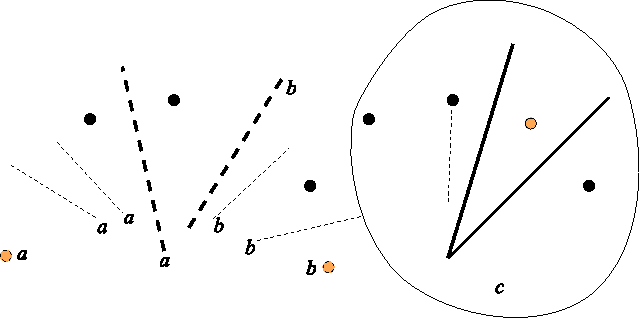
\includegraphics[width=0.97\linewidth]{2009-v2g-08-lah}
\end{center}
\fi
}